% Slides accompanying "Learn RISC-V CPU Implementation and BSV" book
% Copyright (c) 2024 Rishiyur S. Nikhil, All Rights Reserved

% -*- mode: fundamental -*-

% Slides accompanying "Learn RISC-V CPU Implementation and BSV" book
% Copyright (c) 2024 Rishiyur S. Nikhil, All Rights Reserved

% This is a preamble shared by all the slide decks

\documentclass[10pt, aspectratio=169]{beamer}

% \documentclass[17pt]{beamer}

% Avail. font sizes: 8pt, 9pt, 10pt, 11pt, 12pt, 14pt, 17pt, 20pt.
% Default font size is 11pt (= 22pt in full screen mode).

\usepackage{verbatim}
\usepackage{fancyvrb}
\usepackage{listings}

\usepackage{array}

% ================================================================
% Themes

\usetheme{Madrid}          % Line at bottom: Author (affiliation), OptTitle, Conf, page 

% \usetheme{Copenhagen}    % Same as Madrid except bottom line: Author, OptTitle

% \usetheme{Berkeley}    % Takes up 1-inch border on left and top

% ----------------
% colorthemes
% (default), beaver, beetle, seahorse, wolverine

\usecolortheme{seahorse}

% ================================================================
% Customization: show table of contents before each section
% Use \AtBeginSubsection    to show before each subsection

% \AtBeginSection[]
% {
%   \begin{frame}
%     \frametitle{Table of Contents}
%     \tableofcontents[currentsection]
%   \end{frame}
% }

% ================================================================

% ----------------
% The bsc compiler and BSV language
\newcommand{\bsc}{\emph{bsc}}
\newcommand{\BSV}{\bf{BSV}}
% ----------------
% ITALICISE WORDS
\newcommand{\ie}{\emph{i.e.,}}
\newcommand{\eg}{\emph{e.g.,}}
\newcommand{\Eg}{\emph{E.g.,}}
\newcommand{\etc}{\emph{etc.}}
\newcommand{\via}{\emph{via}}
\newcommand{\vs}{\emph{vs.}}

% ----------------
% EMPTY BOXES OF VARIOUS WIDTHS, FOR INDENTATION (N 'em' spaces)

\newcommand{\hm}{\hspace*{1em}}
\newcommand{\hmm}{\hspace*{2em}}
\newcommand{\hmmm}{\hspace*{3em}}
\newcommand{\hmmmm}{\hspace*{4em}}

% ----------------
% Convenient widths (less than text width by N 'em' spaces)

\newlength{\hlessmm}
\setlength{\hlessmm}{\textwidth}
\addtolength{\hlessmm}{-2em}

\newlength{\hlessmmm}
\setlength{\hlessmmm}{\textwidth}
\addtolength{\hlessmmm}{-3em}

\newlength{\hlessmmmm}
\setlength{\hlessmmmm}{\textwidth}
\addtolength{\hlessmmmm}{-4em}

% ----------------
% EMPTY LINES of various heights  (N 'ex' heights)

\newcommand{\vx}{\vspace*{1ex}}
\newcommand{\vxx}{\vspace*{2ex}}
\newcommand{\vxxx}{\cspace*{3ex}}
\newcommand{\vxxxx}{\vspace*{4ex}}

% ----------------
% Inputting verbatim code fragments, with various font sizes

\newcommand{\SHOWCODE}[1]{{\footnotesize\input{#1}}}

\newcommand{\SHOWCODESCRIPT}[1]{{\scriptsize\input{#1}}}

\newcommand{\SHOWCODETINY}[1]{{\tiny\input{#1}}}

% ----------------
% To allow redefinition of "pause" during development vs. deployment
% Argument is vertical space command

% Choose with or without pauses
% \newcommand{\PAUSE}[1]{#1\pause}
\newcommand{\PAUSE}[1]{#1}

% ----------------
% Emojis

\graphicspath{ {./../Figures/} }

\newcommand{\EmojiExercise}{\begin{minipage}[c]{5em}
  \includegraphics[width=3em]
    {person-lifting-weights-emoji-clipart-md-3307277008.png}
\end{minipage}}

% ================================================================
% Title page

\title[Learn CPU design \& {\BSV}]{Learn RISC-V CPU Implementation and {\BSV}}

\subtitle{({\BSV}: a High-Level Hardware Design Language)}

\author[{\copyright} R.S.Nikhil]{Rishiyur S.~Nikhil}
% \institute{Bluespec, Inc.}

% Date is set differently in each slide deck

% \logo{\includegraphics[height=0.6cm]{../Figures/Bluespec_Logo_2022-10}}

% End of preamble
% ****************************************************************


\date{L16: RISC-V: The Fife pipelined CPU}

% ****************************************************************

\begin{document}

% ================================================================

\begin{frame}
 \titlepage

 \begin{center}
  \includegraphics[height=1cm]{Bluespec_Logo_2022-10}
 \end{center}

\end{frame}

% ================================================================

\section{Reminders}

% -*- mode: fundamental -*-

% ================================================================

\begin{frame}[fragile]
\frametitle{Reminders}

\footnotesize

Please git clone: \url{https://github.com/rsnikhil/Learn_Bluespec_and_RISCV_Design} \\
(git pull for latest version).  Repsitory structure:

\vspace{1ex}

\begin{minipage}{0.5\textwidth}\scriptsize
\begin{Verbatim}[frame=single, numbers=left]
    ./Book_BLang_RISCV.pdf
      Slides/
          Slides_01_Intro.pdf
          Slides_02_ISA.pdf
          ...
      Exercises/
          Ex-03-A-Hello-World/
          Ex-03-B-Top-and-DUT/
          ...
      Code/
          src_Top/
          src_Drum/
          src_Fife/
          src_Common/
          ...
      Doc/Installing_bsc_Verilator_etc.{adoc,html}
\end{Verbatim}
\end{minipage}
\hm
\begin{minipage}{0.45\textwidth}
\begin{itemize}

 \item Slides and Exercise are numbered in sync with book Chapter numbers.

 \item For Exercises, please see Appendix E of the book.  Some (not
       all) exercises have associated code in the {\tt Exercises/}
       directory.

\end{itemize}
\end{minipage}

\vspace{2ex}

To compile and run the code for exercises, Drum and Fife, please make sure you have installed:

\begin{itemize}

 \item \emph{bsc} compiler (see \url{https://github.com/B-Lang-org/bsc})

 \item Verilator compiler (see \url{https://www.verilator.org/})
\end{itemize}

\footnotesize

\end{frame}

% ================================================================

\begin{frame}
\frametitle{Chapter Roadmap}

\footnotesize

\begin{center}
\frame{\includegraphics[height=0.825\textheight]{Fig_Chapter_Roadmap}}
\end{center}

\end{frame}

% ================================================================


% ================================================================

\begin{frame}
\frametitle{Flow of information between stages in Drum and Fife}

\label{Slide_Instr_Steps}

\footnotesize

\begin{center}
 \includegraphics[height=0.6\textheight]{Fig_Instr_Exec_w_FIFOs}
\end{center}

\end{frame}

% ================================================================

\begin{frame}
\frametitle{Table of Contents}

\tableofcontents

\end{frame}

% ****************************************************************

\section{Module Interface (same for Drum and Fife)}

\begin{frame}

\begin{center}
  {\LARGE Fife CPU: Module Interface (same for Drum and Fife)}
\end{center}

\end{frame}

% ================================================================

\begin{frame}[fragile]
\frametitle{Module Interface}

\footnotesize


% \SHOWCODE{../Code_Extracts/CPU_IFC.tex}
% TODO: Fix up code-extraction to extract this automatically from source
% from file 'CPU_IFC.bsv' line 27  tag CPU_IFC
{\scriptsize
\begin{Verbatim}[frame=single, numbers=left, label=src\_Common/CPU\_IFC.bsv: line 27 ...]
interface CPU_IFC;
   method Action init (Initial_Params initial_params);

   // IMem
   interface FIFOF_O #(Mem_Req) fo_IMem_req;
   interface FIFOF_I #(Mem_Rsp) fi_IMem_rsp;

   // DMem, speculative
   interface FIFOF_O #(Mem_Req) fo_DMem_S_req;
   interface FIFOF_I #(Mem_Rsp) fi_DMem_S_rsp;
   interface FIFOF_O #(Retire_to_DMem_Commit)  fo_DMem_S_commit;

   // DMem, non-speculative
   interface FIFOF_O #(Mem_Req) fo_DMem_req;
   interface FIFOF_I #(Mem_Rsp) fi_DMem_rsp;

   // Set TIME
   (* always_ready, always_enabled *)
   method Action set_TIME (Bit #(64) t);
endinterface
\end{Verbatim}
}

\vspace{1ex}

The speculative DMem sub-interfaces: \\
\hmm {\tt fo\_DMem\_S\_req} \hmm {\tt fi\_DMem\_S\_rsp} \hmm {\tt fo\_DMem\_S\_commit} \\
were unused in Drum, and are used in Fife.

\end{frame}

% ****************************************************************

\section{Top-level {\tt mkCPU} module}

\begin{frame}[fragile]

\begin{center}
  {\LARGE Fife CPU: Top-level {\tt mkCPU} module}

  \vspace{10ex}

  In file: {\tt Code/src\_Fife/CPU.bsv}
\end{center}

\end{frame}

% ================================================================

\begin{frame}[fragile]
\frametitle{Overall Fife CPU module structure}

\footnotesize

\begin{minipage}{0.725\textwidth}
\begin{Verbatim}[frame=single, label=From src\_Drum/CPU.bsv]
(* synthesize *)
module mkCPU (CPU_IFC);
   // ****************************************************************
   // STATE (sub-modules for pipeline stages)
   ...

   // ****************************************************************
   // STATE (sub-modules for inter-stage connections)

   ...
   // ****************************************************************
   // INTERFACE
   ...
endmodule
\end{Verbatim}
\end{minipage}
\hm
\emph{Details in slides that follow}

\vspace{5ex}

Fife's {\tt mkCPU} module is actually simpler than Drum's {\tt mkCPU}
because the major functionality is now in the separate stage
sub-modules (Drum did not have stage sub-modules).

\end{frame}

% ================================================================

\begin{frame}[fragile]
\frametitle{Fife module state (sub-modules for pipeline stages)}

\footnotesize

\begin{minipage}{0.75\textwidth}
\begin{Verbatim}[frame=single, label=From src\_Fife/CPU.bsv]
   // Pipeline stages
   Fetch_IFC       stage_F          <- mkFetch;
   Decode_IFC      stage_D          <- mkDecode;
   RR_RW_IFC       stage_RR_RW      <- mkRR_RW;
   EX_Control_IFC  stage_EX_Control <- mkEX_Control;  // Branch, JAL, JALR
   EX_Int_IFC      stage_EX_Int     <- mkEX_Int;      // Integer ops
   Retire_IFC      stage_Retire     <- mkRetire;
\end{Verbatim}
\end{minipage}
\hm
\begin{minipage}{0.22\textwidth}
Fife instantiates a sub-module for each of the pipeline stages
\end{minipage}



\end{frame}

% ================================================================

\begin{frame}[fragile]
\frametitle{Fife module state: sub-modules for inter-stage forward-flow connections}

\footnotesize

\begin{minipage}{0.75\textwidth}\scriptsize
\begin{Verbatim}[frame=single, label=From src\_Fife/CPU.bsv]
   // Forward flow connections

   // Fetch->Decode->RR-Dispatch, and direct path RR-Dispatch->Retire
   mkConnection (stage_F.fo_Fetch_to_Decode,  stage_D.fi_Fetch_to_Decode);
   mkConnection (stage_D.fo_Decode_to_RR,     stage_RR_RW.fi_Decode_to_RR);
   mkConnection (stage_RR_RW.fo_RR_to_Retire, stage_Retire.fi_RR_to_Retire);

   // RR-Dispatch->various EX
   mkConnection (stage_RR_RW.fo_RR_to_EX_Control,
		 stage_EX_Control.fi_RR_to_EX_Control);
   mkConnection (stage_RR_RW.fo_RR_to_EX_Int,
		 stage_EX_Int.fi_RR_to_EX_Int);

   // Various EX->Retire
   mkConnection (stage_EX_Control.fo_EX_Control_to_Retire,
		 stage_Retire.fi_EX_Control_to_Retire);
   mkConnection (stage_EX_Int.fo_EX_Int_to_Retire,
		 stage_Retire.fi_EX_Int_to_Retire);
\end{Verbatim}
\end{minipage}
\hm
\begin{minipage}{0.22\textwidth}
Each connection is a FIFO
\end{minipage}

\end{frame}

% ================================================================

\begin{frame}[fragile]
\frametitle{Fife module state: sub-modules for inter-stage backward-flow connections}

\footnotesize

\begin{minipage}{0.75\textwidth}\scriptsize
\begin{Verbatim}[frame=single, label=From src\_Fife/CPU.bsv]
   // Backward flow connections

   // Fetch<-Retire (redirection)
   mkConnection (stage_Retire.fo_Fetch_from_Retire, stage_F.fi_Fetch_from_Retire);
   // RR-Dispatch<-Retire (register writeback)
   mkConnection (stage_Retire.fo_RW_from_Retire, stage_RR_RW.fi_RW_from_Retire);
\end{Verbatim}
\end{minipage}
\hm
\begin{minipage}{0.22\textwidth}
Each connection is a FIFO
\end{minipage}

\end{frame}

% ================================================================

\begin{frame}[fragile]
\frametitle{FIFO connections between separately compiled Fife sub-modules}

\footnotesize

\begin{minipage}{0.22\textwidth}
Each inter-stage FIFO {\tt mkConnection} has this form:
\end{minipage}
\hfill
\begin{minipage}{0.75\textwidth}
\includegraphics[width=\textwidth]{Fig_Composed_FIFO_modularity}
\end{minipage}

\PAUSE{\vspace{2ex}}

\begin{itemize}

 \item Data can traverse from producer to consumer in 1 tick, as
       desired, despite there being two FIFOs, because of the
       semantics of {\tt mkBypassFIFOF} and {\tt mkPipelineFIFOF}
       (Chapter 17).

 \item The structure allows the producer and consumer to be compiled
       independently by \emph{bsc}, with no ``rule-scheduling''
       constraints leaking across stage boundaries.

 \item There are no combinational paths crossing the stage boundary
       (through the two FIFOs).

 \item The structure allows us to reason about correctness of each
       stage completely independently of other stages.

\end{itemize}

\end{frame}

% ================================================================

\begin{frame}[fragile]
\frametitle{Fife module interface definitions}

\footnotesize

\begin{minipage}{0.75\textwidth}\scriptsize
\begin{Verbatim}[frame=single, label=From src\_Fife/CPU.bsv]
   method Action init (Initial_Params initial_params);
      rg_flog <= initial_params.flog;

      stage_F.init (initial_params);
      stage_D.init (initial_params);
      stage_RR_RW.init (initial_params);
      stage_EX_Control.init (initial_params);
      stage_EX_Int.init (initial_params);
      stage_Retire.init (initial_params);
   endmethod

   // IMem
   interface fo_IMem_req = stage_F.fo_Fetch_to_IMem;
   interface fi_IMem_rsp = stage_D.fi_IMem_to_Decode;

   // DMem, speculative
   interface fo_DMem_S_req    = stage_RR_RW.fo_DMem_S_req;
   interface fi_DMem_S_rsp    = stage_Retire.fi_DMem_S_rsp;
   interface fo_DMem_S_commit = stage_Retire.fo_DMem_S_commit;

   // DMem, non-speculative
   interface fo_DMem_req = stage_Retire.fo_DMem_req;
   interface fi_DMem_rsp = stage_Retire.fi_DMem_rsp;

   // Set TIME
   method Action set_TIME (Bit #(64) t) = stage_Retire.set_TIME (t);
\end{Verbatim}
\end{minipage}
\hm
\begin{minipage}{0.22\textwidth}
The {\tt init} method initializes this module and also each stage sub-module.

\vspace{2ex}

The {\tt set\_TIME} method is for updating the {\tt time} CSR.
\end{minipage}

\end{frame}

% ****************************************************************

\section{Fetch stage}

\begin{frame}[fragile]

\begin{center}
  {\LARGE Fife CPU Fetch stage}

  \vspace{10ex}

  In file: \verb|Code/src_Fife/S1_Fetch.bsv|
\end{center}

\end{frame}

% ================================================================

\begin{frame}[fragile]
\frametitle{Fetch stage: interface}

\footnotesize

\begin{minipage}{0.725\textwidth}
\SHOWCODE{../Code_Extracts/Fife_Fetch_IFC.tex}
\end{minipage}
\begin{minipage}{0.25\textwidth}
Interface

\vspace{5ex}

The \verb|FIFO_I| from Retire carries redirection information.

\end{minipage}

\end{frame}

% ================================================================

\begin{frame}[fragile]
\frametitle{Fetch stage: implementation module}

\footnotesize

For module {\tt mkFetch} let us examine file: \verb|Code/src_Fife/S1_Fetch.bsv|

\vspace{4ex}

\begin{itemize}

 \item Rule \verb|rl_Fetch_req| is the forward-flow ``fetching rule'',
       repeatedly invoking \verb|fn_Fetch| to produce IMem requests
       and information for Decode.

       The expression ``\verb|rg_pc+4|'' is, more generally,
       ``\verb|predict(rg_pc)|''.

       In future we can substitute new, improved, predictor functions
       (see book ``Section 18.3.6.4 Better next-PC prediction'').

 \item Rule \verb|rl_Fetch_from_Retire| is the backward-flow.  It
       receives \verb|Fetch_from_Retire| messages from Retire whenever
       Retire needs to change the control flow to something other than
       the predicted PC (due to BRANCH, JAL, JALR, or traps).  This
       rule updates \verb|rg_pc| to the newly specified PC, and also
       updates \verb|rg_epoch|.

 \vspace{4ex}

 \item The expression \verb|(! f_Fetch_from_Retire.notEmpty)|
       in \verb|rl_Fetch_req|'s condition gives it lower priority
       compared to \verb|rl_Fetch_from_Retire| when both are enabled.
       The sooner we perform redirection, the fewer wrong-path
       instructions will be fetched.

\end{itemize}

\end{frame}

% ****************************************************************

\section{Decode stage}

\begin{frame}[fragile]

\begin{center}
  {\LARGE Fife CPU Decode stage}

  \vspace{10ex}

  In file: \verb|Code/src_Fife/S2_Decode.bsv|
\end{center}

\end{frame}

% ================================================================

\begin{frame}[fragile]
\frametitle{Decode stage: interface}

\footnotesize

\begin{minipage}{0.725\textwidth}
\SHOWCODE{../Code_Extracts/Fife_Decode_IFC.tex}
\end{minipage}
\hmm
Interface

\end{frame}

% ================================================================

\begin{frame}[fragile]
\frametitle{Decode stage: implementation module}

\footnotesize

For module {\tt mkDecode} code, let us examine file: \verb|Code/src_Fife/S2_Decode.bsv|

\begin{itemize}

\vspace{4ex}

 \item Rule \verb|rl_Decode| is the forward-flow;
       it repeatedly invokes \verb|fn_Decode| to produce
       information for the next stage.

\end{itemize}

\end{frame}

% ****************************************************************

\section{Register-Read and Dispatch stage (and Register-Write)}

\begin{frame}[fragile]

\begin{center}
  {\LARGE Fife CPU Register-Read and Dispatch stage \\
          (and Register-Write)}

  \vspace{10ex}

  In file: \verb|Code/src_Fife/S3_RR_RW.bsv|
\end{center}

\end{frame}

% ================================================================

\begin{frame}[fragile]
\frametitle{Register-Read and Dispatch stage (and Register-Write): Interface}

\footnotesize

\begin{minipage}{0.725\textwidth}
\SHOWCODE{../Code_Extracts/Fife_RR_RW_IFC.tex}
\end{minipage}
\hfill
\begin{minipage}{0.25\textwidth}
Interface

\vspace{2ex}

The four \verb|FIFO_O| interfaces feed the four execution paths.

\vspace{2ex}

The \verb|FIFO_I| from Retire carries information for register-write
and release of scoreboard reservations.
\end{minipage}

\vspace{2ex}

\verb|rg_oiaat| is used for ``one instruction at a time'' mode, and can be ignored for now.

\end{frame}

% ================================================================

\begin{frame}[fragile]
\frametitle{Register-Read and Dispatch (and Register-Write)  stage: implementation module}

\footnotesize

For module {\tt mkRR\_RW} code, let us examine file: {\tt Code/src\_Fife/S3\_RR\_RW.bsv}

\end{frame}

% ****************************************************************

\section{Execute-Control stage}

% ================================================================

\begin{frame}[fragile]
\frametitle{Execute-Control stage}

\footnotesize

Interface: \hmmmm
\begin{minipage}{0.725\textwidth}
\SHOWCODE{../Code_Extracts/Fife_EX\_Control_IFC.tex}
\end{minipage}

\vspace{5ex}

For module {\tt mkEX\_Control} code, let us examine file: {\tt Code/src\_Fife/S4\_EX\_Control.bsv}

\end{frame}

% ****************************************************************

\section{Execute-Int stage}

% ================================================================

\begin{frame}[fragile]
\frametitle{Execute-Int stage}

\footnotesize

Interface: \hmmmm
\begin{minipage}{0.725\textwidth}
\SHOWCODE{../Code_Extracts/Fife_EX\_Int_IFC.tex}
\end{minipage}

\vspace{5ex}

For module {\tt mkEX\_Int} code, let us examine file: {\tt Code/src\_Fife/S4\_EX\_Int.bsv}

\end{frame}

% ****************************************************************

\section{Retire}

% ================================================================

\begin{frame}[fragile]
\frametitle{Retire}

\footnotesize

Interface: \hmmmm
\begin{minipage}{0.725\textwidth}
\SHOWCODESCRIPT{../Code_Extracts/Fife_Retire_IFC.tex}
\end{minipage}

\vspace{1ex}

For module {\tt mkRetire} code, let us examine file: {\tt Code/src\_Fife/S4\_Retire.bsv}

\end{frame}

% ================================================================

\begin{frame}[fragile]
\frametitle{Some help-functions (2/3)}

\footnotesize

(Help-functions just encapsulate a few actions that are repeated in several places.)

\vspace{5ex}

This function increments the PC and the instruction-number, as we retire each instruction:

\vspace{4ex}

\begin{minipage}{0.725\textwidth}
\SHOWCODE{../Code_Extracts/Drum_redirect.tex}
\end{minipage}

\end{frame}

% ================================================================

\begin{frame}[fragile]
\frametitle{Some help-functions (3/3)}

\footnotesize

(Help-functions just encapsulate a few actions that are repeated in several places.)

\vspace{5ex}

This function records information for later trap-handling:

\vspace{4ex}

\begin{minipage}{0.725\textwidth}
\SHOWCODE{../Code_Extracts/Drum_setup_exc.tex}
\end{minipage}

\end{frame}

% ****************************************************************

\section{top-level FSM}

\begin{frame}[fragile]

\begin{center}
  {\LARGE Fife CPU: top-level FSM}
\end{center}

\end{frame}

% ================================================================

\begin{frame}[fragile]
\frametitle{top-level FSM (1/2)}

\footnotesize

\begin{minipage}{0.725\textwidth}
 \SHOWCODE{../Code_Extracts/Drum_FSM.tex}
\end{minipage}

\vspace{5ex}

The very top-level is very simple and self-evident.

\vspace{2ex}

The {\tt await} statement waits until the {\tt init} method has set
the initial PC, so that we start fetching from the correct address.

\end{frame}

% ================================================================

\begin{frame}[fragile]
\frametitle{top-level FSM (2/2)}

\footnotesize

\begin{minipage}{0.5\textwidth}
 \SHOWCODETINY{../Code_Extracts/Drum_exec_one_instr.tex}
\end{minipage}
\hm
\begin{minipage}{0.45\textwidth}
 This is practically a direct coding of the instruction-execution steps
 in the diagram on Slide~\ref{Slide_Instr_Steps}.
\end{minipage}


\end{frame}

% ****************************************************************

\section{FSM Fetch step}

\begin{frame}[fragile]
\frametitle{FSM Fetch step}

\footnotesize

\begin{minipage}{0.75\textwidth}
 \SHOWCODE{../Code_Extracts/Drum_Fetch.tex}
\end{minipage}
\hm
\begin{minipage}{0.2\textwidth}
 Just invokes {\tt fn\_Fetch} and sends the two results into a register for Fetch and
 into a FIFO for IMem memory.
\end{minipage}

\end{frame}

% ****************************************************************

\section{FSM Decode step}

\begin{frame}[fragile]
\frametitle{FSM Decode step}

\footnotesize

\begin{minipage}{0.75\textwidth}
 \SHOWCODE{../Code_Extracts/Drum_Decode.tex}
\end{minipage}
\hm
\begin{minipage}{0.2\textwidth}
 Just invokes {\tt fn\_Decode} on the inputs from Fetch and memory,
 and sends the result into a register for Register-Read-and-Dispatch.
\end{minipage}

\end{frame}

% ****************************************************************

\section{FSM Register-Read and Dispatch step}

\begin{frame}[fragile]
\frametitle{FSM Register-Read and Dispatch step}

\footnotesize

\begin{minipage}{0.75\textwidth}
 \SHOWCODE{../Code_Extracts/Drum_RRD.tex}
\end{minipage}
\hm
\begin{minipage}{0.2\textwidth}
 Using input from Decode, reads two registers {\tt rs1} and {\tt rs2};
 then invokes {\tt fn\_Dispatch}, and
 and sends the result into a register for the Execute stage.
\end{minipage}

\end{frame}

% ****************************************************************

\section{FSM Execute and Retire step}

\begin{frame}[fragile]

\begin{center}
  {\LARGE Fife CPU: FSM Execute and Retire step}
\end{center}

\end{frame}

% ================================================================

\begin{frame}[fragile]
\frametitle{FSM Execute and Retire step flows}

\begin{minipage}{0.75\textwidth}
 \includegraphics[width=\textwidth]{Fig_Retire_Layers_1}
\end{minipage}
\hm
\begin{minipage}{0.2\textwidth}
4 possible flows.
\begin{itemize}
 \item Direct
 \item Control
 \item Int
 \item DMem
\end{itemize}

\vspace{2ex}

Each ultimately resulting in up to 3 possible actions.
\end{minipage}

\end{frame}

% ================================================================

\begin{frame}[fragile]
\frametitle{Updating the {\tt minstret} CSR (counting instructions retired)}

\footnotesize

The {\tt minstret} CSR is incremented for each instruction retired.

\emph{Except:}

\begin{itemize}

 \item An instruction that raises an exception.

 \item A CSRRxx instruction that writes a value into {\tt minstret}.

\end{itemize}

\vspace{2ex}

We increment using:
\begin{tabbing}\tt
\hmm  csrs.ma\_incr\_instret;
\end{tabbing}

\vspace{2ex}

The {\tt minstret} and {\tt mcycle} CSRs are useful in performance
measurement (instructions/cycle).

\end{frame}

% ================================================================

\begin{frame}[fragile]
\frametitle{Execute and Retire Direct flow (1/4)}

\footnotesize

\begin{minipage}{0.725\textwidth}
\begin{Verbatim}[frame=single, label=From src\_Drum/CPU.bsv]
   Action a_Retire_direct =
   action
      let x_direct = rg_Dispatch.to_Retire;
      if (x_direct.exception) begin
	 fa_setup_exception (x_direct.pc,        // epc
			     x_direct.cause,     // cause
			     x_direct.tval);     // tval
	 log_Retire_Direct_exc (rg_flog, x_direct);
      end
      // ----------------
      ...
\end{Verbatim}
\end{minipage}

\end{frame}

% ================================================================

\begin{frame}[fragile]
\frametitle{Execute and Retire Direct flow (2/4)}

\footnotesize

\begin{minipage}{0.725\textwidth}
\begin{Verbatim}[frame=single, label=From src\_Drum/CPU.bsv]
      ...
      // ----------------
      else if (is_legal_CSRRxx (x_direct.instr)) begin
	 match { .exc, .rd_val } <- csrs.mav_csrrxx (x_direct.instr,
						     x_direct.rs1_val);
	 if (exc)
	    fa_setup_exception (x_direct.pc,                  // epc
				cause_ILLEGAL_INSTRUCTION,    // cause
				x_direct.instr);              // tval
	 else begin
	    fa_update_rd (x_direct, rd_val);
	    fa_redirect_Fetch (x_direct.fallthru_pc);
	 end
	 log_Retire_CSRRxx (rg_flog, exc, x_direct);
      end
      // ----------------
      ...
\end{Verbatim}
\end{minipage}

\end{frame}

% ================================================================

\begin{frame}[fragile]
\frametitle{Execute and Retire Direct flow (3/4)}

\footnotesize

\begin{minipage}{0.725\textwidth}
\begin{Verbatim}[frame=single, label=From src\_Drum/CPU.bsv]
      ...
      // ----------------
      else if (is_legal_MRET (x_direct.instr)) begin
	 fa_redirect_Fetch (csrs.read_epc);
	 csrs.ma_incr_instret;
	 log_Retire_MRET (rg_flog, x_direct);
      end
      // ----------------
      ...
\end{Verbatim}
\end{minipage}

\end{frame}

% ================================================================

\begin{frame}[fragile]
\frametitle{Execute and Retire Direct flow (4/4)}

\footnotesize

\begin{minipage}{0.725\textwidth}
\begin{Verbatim}[frame=single, label=From src\_Drum/CPU.bsv]
      ...
      // ----------------
      else if (is_legal_ECALL (x_direct.instr)
	       || is_legal_EBREAK (x_direct.instr))
	 begin
	    let cause = ((x_direct.instr [20] == 0)
			 ? cause_ECALL_FROM_M
			 : cause_BREAKPOINT);
	    fa_setup_exception (x_direct.pc,    // epc
				cause,
				0);             // tval
	    csrs.ma_incr_instret;
	    log_Retire_ECALL_EBREAK (rg_flog, x_direct);
	 end
      else begin
	 wr_log2 (rg_flog, $format ("CPU.EX.Direct: IMPOSSIBLE"));
	 $finish (1);
      end
   endaction;
\end{Verbatim}
\end{minipage}

\end{frame}

% ================================================================

\begin{frame}[fragile]
\frametitle{Execute and Retire Control flow}

\footnotesize

\begin{minipage}{0.725\textwidth}
\begin{Verbatim}[frame=single, label=From src\_Drum/CPU.bsv]
   Action a_EX_Control =
   action
      let x = rg_Dispatch.to_EX_Control;
      let y <- fn_EX_Control (x, rg_flog);
      rg_EX_Control_to_Retire <= y;
      ...
   endaction;
\end{Verbatim}
\end{minipage}

\begin{minipage}{0.725\textwidth}
\begin{Verbatim}[frame=single]
   Action a_Retire_Control =
   action
      let x_direct  = rg_Dispatch.to_Retire;
      let x_control = rg_EX_Control_to_Retire;
      if (x_control.exception)
	 fa_setup_exception (x_direct.pc,
			     x_control.cause,
			     x_control.tval);
      else begin
	 fa_update_rd (x_direct, x_control.data);
	 fa_redirect_Fetch (x_control.next_pc);
	 csrs.ma_incr_instret;
      end
      ...
   endaction;
\end{Verbatim}
\end{minipage}

\end{frame}

% ================================================================

\begin{frame}[fragile]
\frametitle{Execute and Retire Int flow}

\footnotesize

\begin{minipage}{0.725\textwidth}
\begin{Verbatim}[frame=single, label=From src\_Drum/CPU.bsv]
   Action a_EX_Int =
   action
      let x = rg_Dispatch.to_EX;
      let y <- fn_EX_Int (x, rg_flog);
      rg_EX_to_Retire <= y;
      ...
   endaction;
\end{Verbatim}
\end{minipage}

\begin{minipage}{0.725\textwidth}
\begin{Verbatim}[frame=single]
   Action a_Retire_Int =
   action
      if (rg_EX_to_Retire.exception)
	 fa_setup_exception (rg_Dispatch.to_Retire.pc,
			     rg_EX_to_Retire.cause,
			     rg_EX_to_Retire.tval);
      else begin
	 fa_update_rd (rg_Dispatch.to_Retire, rg_EX_to_Retire.data);
	 fa_redirect_Fetch (rg_Dispatch.to_Retire.fallthru_pc);
	 csrs.ma_incr_instret;
      end
      ...
   endaction;
\end{Verbatim}
\end{minipage}

\end{frame}

% ================================================================

\begin{frame}[fragile]
\frametitle{Execute and Retire DMem flow (1/2)}

\footnotesize

\begin{minipage}{0.725\textwidth}
\begin{Verbatim}[frame=single, label=From src\_Drum/CPU.bsv]
   Action a_EX_DMem =
   action
      Mem_Req y = rg_Dispatch.to_EX_DMem;
      f_DMem_req.enq (y);
      ...
   endaction;
\end{Verbatim}
\end{minipage}

\end{frame}

% ================================================================

\begin{frame}[fragile]
\frametitle{Execute and Retire DMem flow (2/2)}

\footnotesize

\begin{minipage}{0.725\textwidth}\scriptsize
\begin{Verbatim}[frame=single, label=From src\_Drum/CPU.bsv]
   Action a_Retire_DMem =
   action
      let x_direct = rg_Dispatch.to_Retire;
      let mem_rsp <- pop_o (to_FIFOF_O (f_DMem_rsp));
      Bool exception = ((mem_rsp.rsp_type == MEM_RSP_ERR)
			|| (mem_rsp.rsp_type == MEM_RSP_MISALIGNED));
      if (exception) begin
	 Bit #(4) cause = ((mem_rsp.rsp_type == MEM_RSP_MISALIGNED)
			   ? (is_LOAD (x_direct.instr)
			      ? cause_LOAD_ADDRESS_MISALIGNED
			      : cause_STORE_AMO_ADDRESS_MISALIGNED)
			   : (is_LOAD (x_direct.instr)
			      ? cause_LOAD_ACCESS_FAULT
			      : cause_STORE_AMO_ACCESS_FAULT));
	 fa_setup_exception (x_direct.pc,                 // epc
			     cause,
			     truncate (mem_rsp.addr));    // tval
      end
      else begin
	 fa_update_rd (x_direct, truncate (mem_rsp.data));
	 fa_redirect_Fetch (x_direct.fallthru_pc);
	 csrs.ma_incr_instret;
      end
      ...
   endaction;
\end{Verbatim}
\end{minipage}

\end{frame}

% ================================================================

\begin{frame}[fragile]
\frametitle{action for exceptions}

\footnotesize

\begin{minipage}{0.725\textwidth}
\begin{Verbatim}[frame=single, label=From src\_Drum/CPU.bsv]
   Action a_exception =
   action
      Bool is_interrupt = False;
      Bit #(XLEN) tvec_pc <- csrs.mav_exception (rg_epc,
						 is_interrupt,
						 rg_cause,
						 rg_tval);
      rg_exception <= False;
      fa_redirect_Fetch (tvec_pc);
      ...
   endaction;
\end{Verbatim}
\end{minipage}

\end{frame}

% ****************************************************************

\section{Final Comments}

\begin{frame}[fragile]
\frametitle{{\BSV}: {\tt StmtFSM} final comments}

\footnotesize

Fife CPU code, using {\tt StmtFSM}, looks just like a C/C++ program
with somewhat different syntax.

\vspace{2ex}

So: can't we just code it in C/C++ and compile that to hardware?

\vspace{2ex}

\begin{itemize}
        
 \item Difficult to compile \emph{general-purpose} C into hardware.

       C has many constructs that have no obvious mapping into
       hardware, such as pointers, the address-of operator ``\&'',
       address arithmetic, malloc, and so on.

       But can’t we define a restricted subset of C suitable for
       hardware design?

       Compilation is still very difficult: no distinction between
       variables used to hold state (registers) {\vs} variables used
       to hold temporary intermediate values (wires); no distinction
       between pure and side-effect constructs; ...

 \item No concurrency.  It may be possible to compile a subset of C to
       hardware, similar to Drum.  But this is the easy case
       (completely sequential).  Very hard to generalize to pipelines
       and more concurrent implementations (Fife, and beyond).

\end{itemize}

\end{frame}

% ****************************************************************

% -*- mode: fundamental -*-

% Slides accompanying "Learn RISC-V CPU Implementation and BSV" book
% Copyright (c) 2024 Rishiyur S. Nikhil, All Rights Reserved

% This is a postamble shared by all the slide decks

% ================================================================

\begin{frame}

\begin{center}
  {\LARGE End}
\end{center}

\end{frame}

% ================================================================


% ****************************************************************

\end{document}
% ****************************************************************
